\section{Electronics Design}

The electronics for Roxi can be broken into three major categories: Senors, Power, and computers.

\subsection{Sensors}

Roxi uses vision and LIDAR as its primary sensors used for the navigation challenge and also has GPS and wheel encoders to allow for waypoint navigation.

\subsubsection{Vision}

The vision system consists of a AVT Guppy F-036C camera connected via an IEEE 1394a link to the main computer. This camera is capable of 752 x 480 resolution at 64 fps. This camera is polled at approximately 10 Hz to send a new frame to the vision algorithm.  The camera is placed at the top of the mast, facing forwards and down to allow the lines and obstacle in front of the robot to be sensed.

\subsubsection{Wheel Encoder}

Each wheel is connected to a quadrature wheel encoder, allowing wheel rate to be measured. This allows the velocity of the robot to be measured. The encoder is a US Digital E3-200-375-I-H-M-B, with 200 counts per revolution and an index channel. This allows for wheel rates up to XX speed to be sensed. The quadrature lines drive interrupts on a microcontroller, which then feeds the state of the lines to a state machine which increments or decrements a wheel counter. Wheel angular velocity is measured by differencing the number of counts over a 5 ms period, allowing a bandwidth of XX Hz and XX m / s. The microcontrollers are capable of sending both rate and count information to the laptop, allowing for speed control and odometry operations.

\subsubsection{LIDAR}

Two front and rear mounted Sick NAV300 LIDAR are used as object and ramp detectors. The LIDAR have a $270^{\circ}$ FOV and a 10 meter range. The front facing LIDAR is used as an object finder, while the back facing LIDAR is used as a safety feature allowing the robot to sense if an object / person is moved behind it after the robot has moved through an area.

\subsubsection{GPS}

A GPS is used to provide world position to the robot, allowing obstacles to be placed in world space and allowing waypoints to be followed. A Garmin ``GPS 18-5Hz'' gps is mounted to the mast to allow a clear view of the sky. This GPS is accurate to $<15$ m / $<3$ m (GPS / WAAS) and has a time to first fix of 45 seconds. The GPS updates 5 times per second.

\subsection{Power}

\begin{figure}[H]
\begin{center}
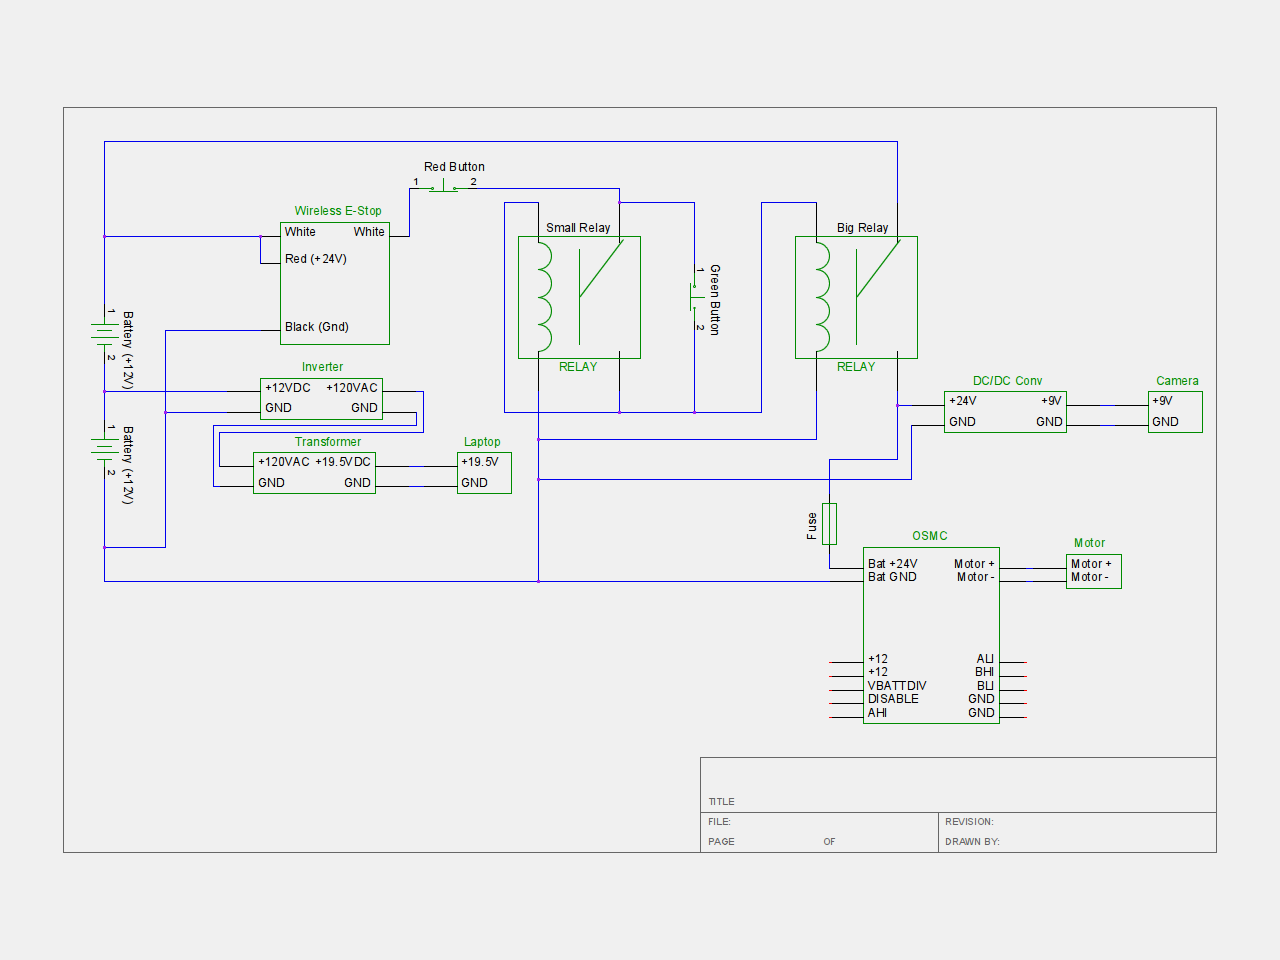
\includegraphics[width=6in]{./igvc_power.png}
\caption{Power Schematic}
\label{FIG:Power}
\end{center}
\end{figure}

\subsubsection{Main Power}

Main power for the robot comes from two sealed lead acid gell-cell batteries. These batteries are connected in series to produce a nominal 24 VDC supply for the motors and other systems. This provides approximately XX $W \cdot hr$ of energy, XX hours of runtime of the motors, and XX hours of runtime of the electronics and motors.

The batteries are connected to a power distribution board, which allows the connection to each motor to be fused with XX Amps, allowing power to be cut in the event of a motor stall to prevent damage to the H-bridge. Power is also provided to several DC-DC boost converters, which output 5 VDC, 9 VDC, and 19.5 VDC for other electronics on the robot.

\subsubsection{H Bridge}

Each motor is connected to an OSMC H-bridge. This board is used to allow a low power signal from the microcontrollers to generate a high power PWM input to the motors. Each OSMC is capible of switching up to 50 VDC at 160A cont / 300A peak, allowing significant margin above our standard operating power of around 24 VDC / 20 A.

\subsubsection{Component Power}

Other systems are provided power through the use of DC-DC converters to produce voltages at 5 V, 9 V, and 19.5 V. This allows for the usb tethered microcontrollers, the sensors, and the main computer to be powered off of the main lead acid batteries. This greatly simplifies charging the robot, as only one battery system needs to be maintained.

\subsection{Computers}

\subsubsection{Main Computer}

Nearly all computation is performed on a single laptop containing a quadcore Intel Core i7 cpu, cuda enabled NVIDIA 285M gpu, and 6 GB of RAM. This computer is responsible for all vision, LIDAR, and GPS data processing and all path planning and control algorithms. It also forms the core of the sensor interconnects, providing the firewire and USB bus the camera, GPS, and microcontrollers use. This laptop replaces the main computer used in previous years, and was replaced with support from Northrup Grumman.

\subsubsection{MCU}

Microcontrollers are used on Roxi as data acquisition boards to collect data from the wheel encoders, and as motor control boards to generate PWM signals to drive the H-bridges. There are 6 ATmega328p based Arduino Duemilanove boards on the robot, 4 interfacing with the wheel encoders, and 2 to drive the motors.

\subsection{Safety Features}

As autonomous systems are dangerous, and can behave unpredictably when hardware or software errors occur, several safty features are included in this robot.

\subsubsection{Emergancy Stop}

The robot is equiped with an emergency stop that when triggered will physically disconnect power to the motors. This will stop forward motion quickly. Both a physical button on the back of the robot and a wireless trigger are provided.

\subsubsection{Safety Light}



\subsubsection{Rear-Facing LIDAR}

This robot also uses a rear facing LIDAR as a saftey feature. This allows the robot to sense if something has moved behind it, allowing the robot to avoid hitting anyone walking behind it if the robot decides to move backwards during autonomous operation.
